\section{Introduction}
\label{sec:Introduction}

This is a summary of the electronic text-book \cite{PACGGHSY} with comments and a little rewritten sections by the author and based on the peers and supervisor's feedback. 
Other references are marked. 
This summary aims to be give a clear instruction of the usage and applicability of Coq.\\

\subsection{Preface}
\label{subsec:preface}

Within this introduction the mathematical underpinning of reliable software is given.
The building blocks are

\textcolor{red}{!!!TODO!!!}

\begin{itemize}
\item basics concepts of logic (see sec. \ref{} % TODO:)
\item computer assisted theorem proving (see sec. \ref{} %TODO:)
\item Coq-proof assistant (see sec. \ref{} %TODO:
\item functional programming (see sec. \ref{} %TODO)
\item operational semantics (see sec. \ref{} %TODO:)
\item logics for reasoning about programs (see sec. \ref{} %TODO: )
\item static type systems (see sec. \ref{} %TODO:)
\end{itemize} 


\subsection{Overview}
\label{subsec:Overview}

There is a lot of motivation for reliable software. 
First of all the scale, complexity and number of involved people in modern systems is increasing.
Therefore building correct software is extremely difficult.
Information processing is waved into every aspect of society, leading to amplified costs of bugs and insecurities upto multiple levels. An on the hand rule says the later an error is located the more expensive it is.\\
Computer scientists and software engineers have responded to improve reliability with a lot of design threats and to improve reliability and mathematical technices for reasoning.
Within this work it should be contributed to validates these properties. 
They are:
\begin{enumerate}
\item basic tools from logic for making and justifying precise claims about programs
\item use of proof assistants to construct rigorous logical arguments
\item functional programmings as method of programming and simplifying reasoning about programs as a bridge between programming and logic
\end{enumerate}



\subsection{Logic}
\label{subsec:logic}

\begin{quote}
``As a matter of fact, logic has turned out to be significantly more effective in computer science then it has been in mathematics.'' \cite{PACGGHSY} 
\end{quote}
Volumes have been written about the central role of logic in computer science. 
It's fundamental tool {\itshape inductive proof} is going to be explored very deeply within this work.


\subsection{Proof Assistants}
\label{subsec:proofassistants}

In computer science proof assistants are an important tool for helping construct formal proofs of logical propositions.
There are two categories of these tools.\\
First of all there are automated theorem proofers. 
These are able of a ''push-button- operation'' which returns true, false'' or ``ran out of time'' given a proposition.
Example applications are \glspl{SAT-solver}, \glspl{SMT-solver} or \glspl{model checker}. 
Second there are proof assistants, which are hybrid tools that automate the more routine-like aspects of a proof, while depending on human guidance. 
Examples are \gls{Isabelle}, Agda, Twelf, ACL2, PVS or Coq.\\
The Coq proof assistant has been developed since 1983 and gathered a large community in research and industry.
It provides a rich environment for interactive development of machine-checked code for formal reasoning.\\
It's kernel is a simple proof checker, ensuring that correct dilution of sets are ever performed. 
Moreover, there are high-level facilities for proof development.
Coq has been applied as critical enabler across computer science and mathematics a platform for modeling programming languages and as an environment for developing {\itshape formally certified software and hardware}.
 

\subsection{Trivia}
\label{subsec:trivia}

Some French computer scientist have a tradition of naming their software as animal species.
{\itshape Coq} is the French word for roster, which is the national symbol of France.
Coq sounds like the initial of the \gls{CoC}.
One of Coq's early developers is called Terry Coquand.


\subsection{Functional Programming}
\label{subsection:functionalProgramming}

There are two meanings of the term. 
It is either refereed to programming idioms (something like a pattern) or something else as in this work.\\

Functional programming refers to a way of programming, which is free of side effects.
By side effects phenomena as I/O or redirecting pointers are meant. 
For example, let's imagine iterative sorting. 
A sorting-function might take a list of numbers and rearrange the pointers to these numbers.
In functional programming a new list is returned which contains the same number arranged in an order.\\ 
Advantages of functional programming are that we are having a new data structure leaving the old one intact. 
Therefore there is no reason to worry about the structure being shared, whether one part of the program might break an invariant that another part of the program relies on.\par
The industry is interested in functional programming due to it's simple behavior in the presence of accuracy.
Furthermore, functional programming is more easy to parallelize then the counter parts.
For example the map-reduce idiom, which relies at the heart of massively distributed query processor like \gls{Hadoop} is functional programming. 

\begin{quote}
`` [...] When we come to look more closely, we find that these two sides of Coq are actually aspects of the very same underlying machinery - i.e. proofs are programs.'' 
\end{quote}




\subsection{System Requirements}
\label{subsection:systemrequirements}

Coq runs on Windows, Linux and macOS.
A current installation can be found on the Coq-homepage \cite{Coq}. 
The listings in this work from \cite{PACGGHSY} have been tested using Coq 8.8.1.
The following choices of integrated development environments (IDEs) are available. 


\paragraph{Coq in the command line}
\label{par:CoqInTheCommandLine}

It is not recommended to use Coq in the command line mode. 
Because the interactive mode is preferred, when using Coq as a proof assistant. 


\paragraph{Proof General}
\label{par:proofGeneral}

Proof general is an Emacs based IDE. 
It is recommended to users who are familiar with the Emacs-editor.
Proof general supports multipel proof assistants. 
The corresponding proof general mode,  the socalled \lstinline!Coq-mode!, will be invoted automatically when a proof script a \lstinline!v.!-file is opened \cite{PROOFGENERAL}. 


\paragraph{CoqIDE}
\label{par:CoqIDE}

CoqIDE is a simple stand-alone IDE. 
It labels itself as a user-friendly replacement to \lstinline!coqtop! \cite{COQIDE}.   
It should be available with any Coq-installation. 
It shall be warned that CoqIDE should be run with the asynchronous and error reliance model disabled. 

\paragraph{Coquille}
\label{par:Coquille}

Coquille is a vim plug-in used by the author.
It can be found at \url{https://github.com/Werner2005/coquille}.
It provides syntax check by color highlighting and and interactive evaluation.  
The author worked with coquille to explorer Coq.\\
It provides a similar workflow as CoqIDE. 
Coquille labels itself as a user friendly  replacement of \lstinline!coqtop!. 
The running buffer is the one where navigation takes place. 
To that coquille provides forwards and backwards navigation.\\

In order to launch coquille open a Coq script (a \texttt{.v}-file) by gvim or vim from the console and run (\texttt{:CoqLaunch}). 
Coqille's main screen provides an evaluation of the Coq-code untill the position of the curser (press \texttt{F4}), a stepwise forward (press \texttt{F2}) and backwards (press \texttt{F3}) evaluation.                 
Furthermore, the plug-in provides syntax highlighting (see Figure \ref{fig:Coquille}).
While running a buffer it is deposited grey.
A green deposition indicates a correct evaluation. 
And a just proven subgoal is displayed in the goal window. 
Failing commands are deposited red and the message window reports errors.


\paragraph{Encoding}
\label{par:encoding}

Coq proof scripts (\texttt{.v}-files) are encoded by ASCII. But support for unicode is provided, too \cite{GallinaSpec}.


\begin{figure}[h]
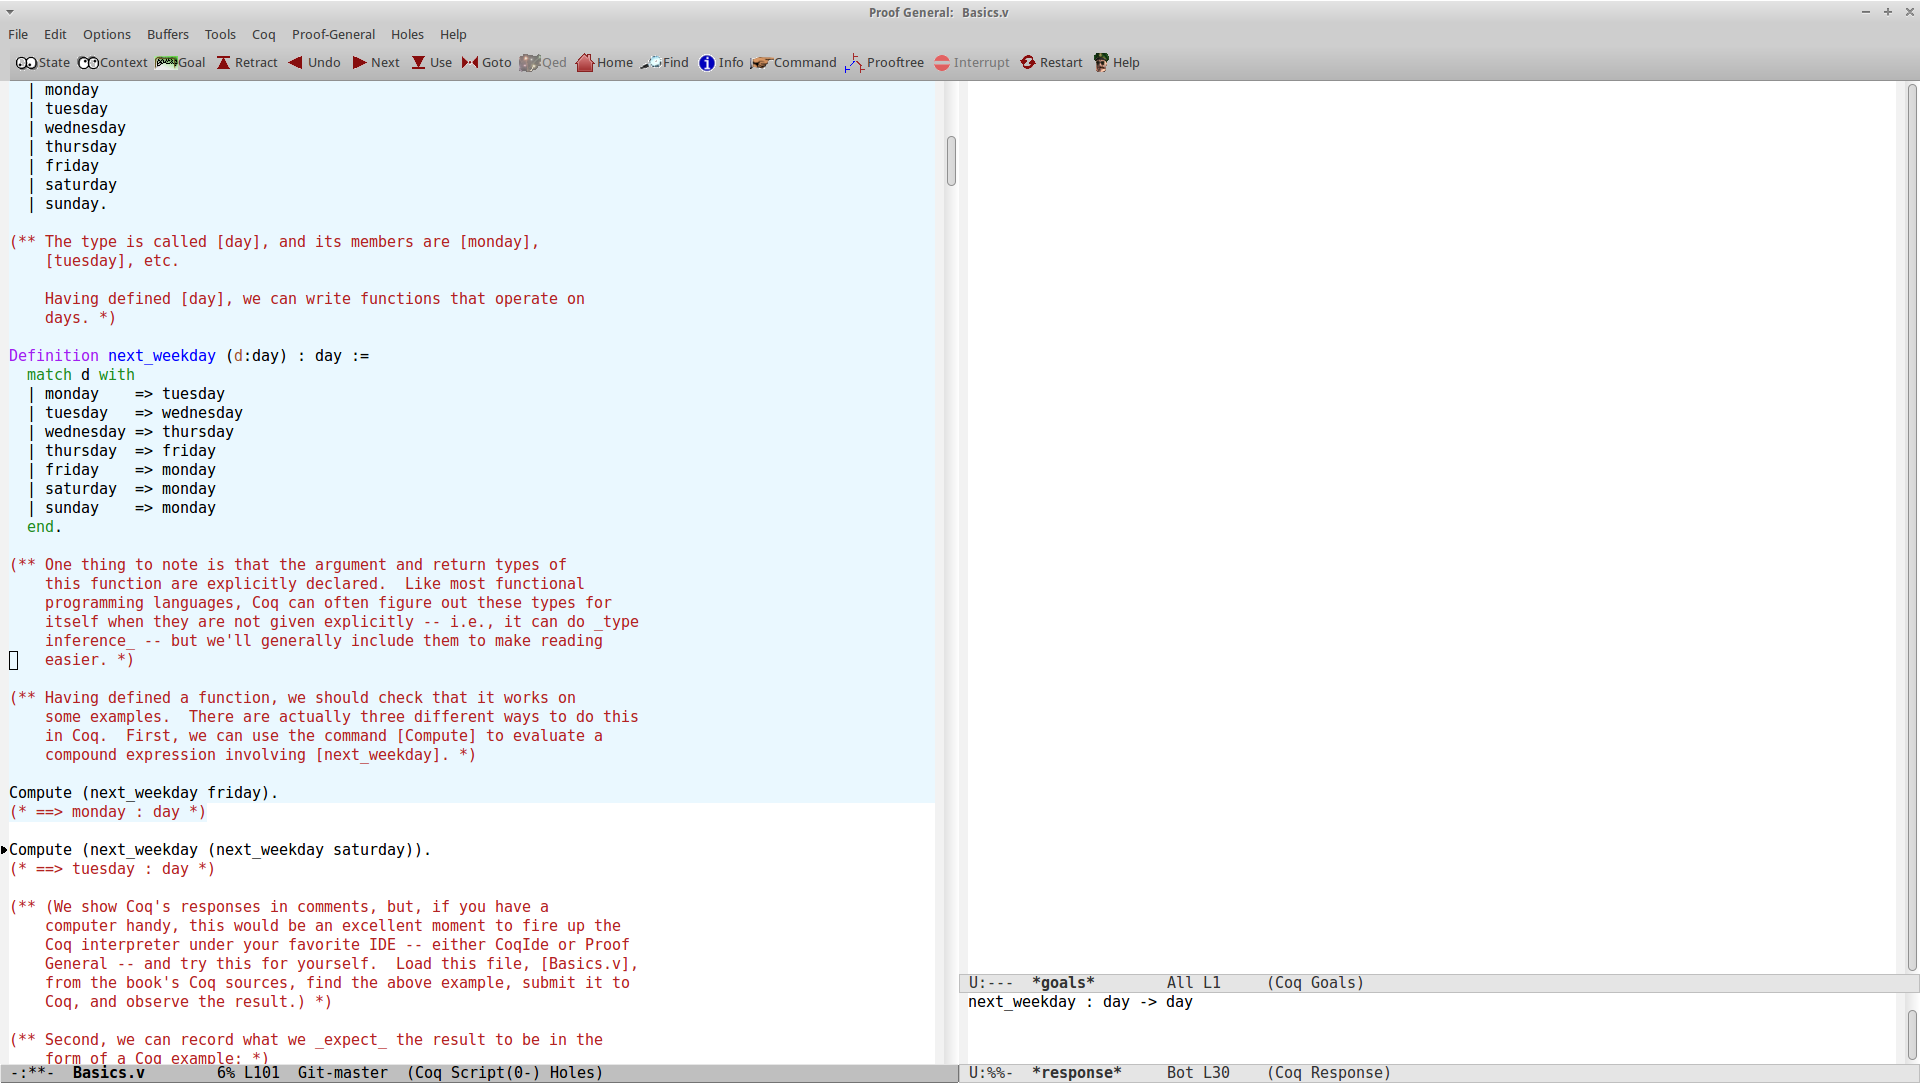
\includegraphics[width=0.9\textwidth]{proofgeneral.png}
\caption{Coq interface launched in gvim using coquille.\\ 
Left window: The open Coq-script \texttt{Basics.v}.
Upper right: The {\itshape goal window}. 
Lower right: The {\itshape message window} \cite{COQIDE}.}
\label{fig:proofGeneral}
\end{figure}


\subsection{Languages}
\label{subsec:languages}

Coq uses three different languages. 
First, there is a vernacular language. 
It is a top-level interaction. 
It's keywords start with a capital letter e.g. \lstinline!Theorem!, \lstinline!Proof! and  \lstinline!Qed!. 
Second, there is the tactics language (e.g. \lstinline!intros! and \lstinline!exact!).
Finally there is an unnamed language of Coq-terms. 
It consists of a lot of operators (e.g. \lstinline!for all A:Prop, A -> A!).
Technically, it is part of the tactics language, but it is useful to think of it as it's own thing \cite{coq}.
\url{https://coq.inria.fr/refman/language/gallina-specification-language.html}